\documentclass{beamer}
\usetheme{Pittsburgh}
\beamertemplatenavigationsymbolsempty


\usepackage{amsmath}
\usepackage{amssymb}
\usepackage{bm} % For bold math symbols
\usepackage{graphicx}


\usepackage{subfigure}
\usepackage{multirow}
\usepackage{multicol}
\usepackage{color}
\usepackage{url}
\usepackage{hyperref}
\usepackage{listings}
\usepackage{algorithm}
\usepackage{physics}
% add image path
\graphicspath{{../Images/}}

\title{Overview of the results\\
\tiny{Wednesday, 05 February 2025}}
\author{Andrea Bonifacio}
\date{}

\begin{document}

\begin{frame}
\titlepage
\end{frame}


\begin{frame}{Brief recap}

    \textbf{The idea}
    \begin{itemize}
        \item Integrate insights from accurate simulations into less accurate ones to achieve:
        \begin{itemize}
            \item Comparable accuracy.
            \item Drastically reduced computational time.
        \end{itemize}
        \item \textbf{Transparent}: Avoids black-box methodologies.
    \end{itemize}
    
    \vspace{0.5cm}
    
    \end{frame}

% \begin{frame}
% \frametitle{Goal}
% \begin{columns}
%     \column{0.5\textwidth}
%     The \textbf{ideal} method should be:
%     \begin{itemize}
%     \item Geometry-independent.
%     \item Topology-independent.
%     \item Not a black-box.
%     \item Fast.
%     \end{itemize}
%     \column{0.5\textwidth}
%     The proposed method is:
%     \begin{itemize}
%     \item[] X
%     \item[] \checkmark
%     \item[] \checkmark
%     \item[] \checkmark
%     \end{itemize}
% \end{columns}
% \end{frame}





\begin{frame}
\frametitle{Suggestions}
\begin{itemize}
    \item Test a more complex geometry.
    \item Study the effect of dataset size on the model performance.
    \item Evaluate the role of message-passing in the accuracy of the model.
\end{itemize}
\end{frame}

\begin{frame}
\frametitle{New geometry}
\begin{itemize}
    \item A new geometry has been developed to test the limits of this method. 
    \item Mixed boundary conditions to fix in place only half of the base.
    \item Built to capture ``high frequency behavior'' such as a beam moving because the baseplate is not fixed.
\end{itemize}
\end{frame}

\begin{frame}
\frametitle{New geometry}
\begin{columns}
    \column{0.5\textwidth}
    \begin{figure}
        \centering
        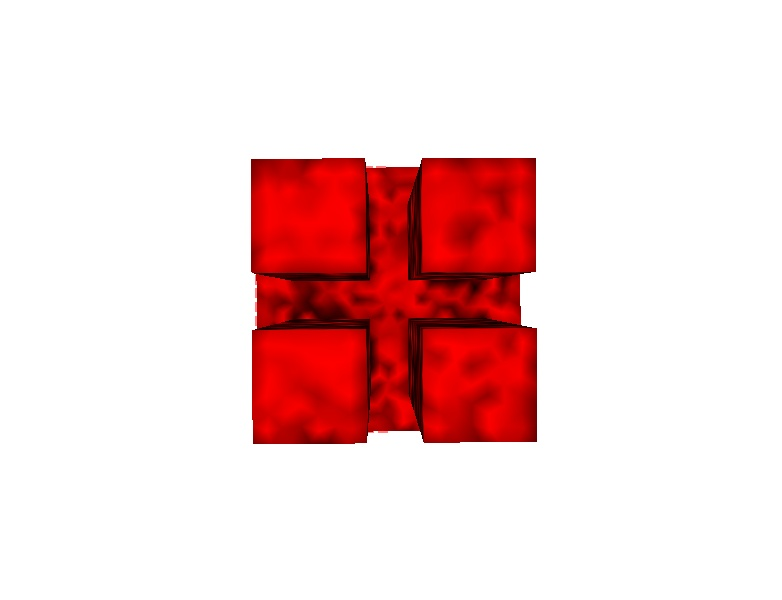
\includegraphics[width=0.95\textwidth]{Images/complex_domain_topview.png}
        \caption{Top view of the new geometry}
    \end{figure}
    \column{0.5\textwidth}
    \begin{figure}
        \centering
        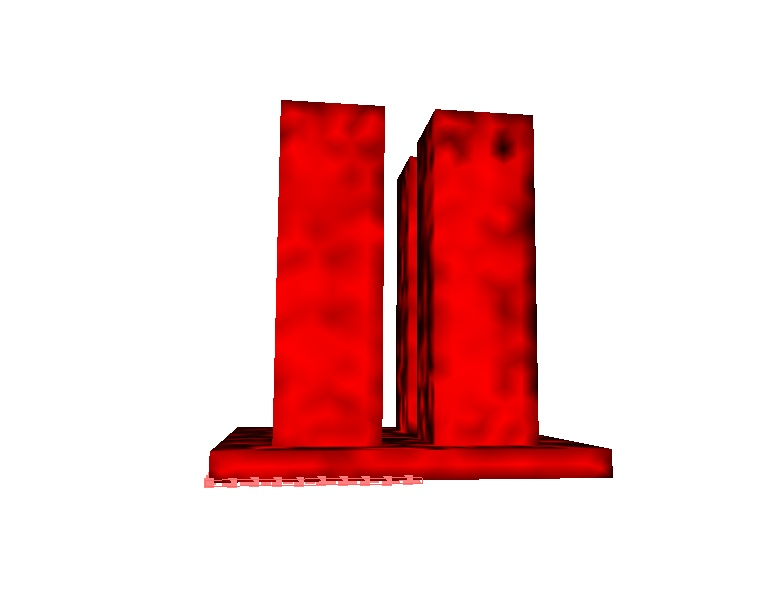
\includegraphics[width=0.95\textwidth]{Images/complex_domain_side.png}
        \caption{Side view of the new geometry}
    \end{figure}
\end{columns}
\end{frame}

\begin{frame}
\frametitle{New geometry}
The new geometry consists in 4 beams attached to a baseplate.
\begin{itemize}
    \item Half of the baseplate is fixed in place, meaning that the beams on that side behaves similarly to beams fixed on one end.
    \item The other half of the plate is free to move, meaning that the beams on that side behaves similarly to beams fixed on both ends.
    \item ``High frequency behavior'' arises when force is applied only on one beam, but the others move a bit in the high resolution simulation.
    \end{itemize}
\end{frame}


\begin{frame}
\frametitle{Datasets}
    \begin{itemize}
        \item Three datasets have been created to see the effect of dataset size on the model performance.
        \begin{itemize}
            \item Small dataset: 2000 simulations.
            \item Medium dataset: 5000 simulations.
            \item Large dataset: 10000 simulations.
        \end{itemize}
    \end{itemize}
\end{frame}

\begin{frame}{Networks}
    \begin{itemize}
        \item Two different networks have been tested:
        \begin{itemize}
            \item A Graph-Neural Network (GNN), with different numbers of message-passing layers (3, 5, 9)
            \item A Fully Connected (FC) network.
        \end{itemize}
    \end{itemize}
\end{frame}
    
            

\begin{frame}
    \frametitle{Numerical Results}
    \begin{itemize}
        \item Each model has been tested on the three datasets, with a live testing. After the training, each model has been put in a simulation environment where its predictions are compared to the fine solution.
        \item After the testing, the following metrics have been computed:
        \begin{itemize}
            \item Root Mean Squared Error (RMSE).
            \item MSE
            \item Adimensionalized RMSE (RMSE divided by the length of the domain).
        \end{itemize}
    \end{itemize}
\end{frame}

\begin{frame}
    \frametitle{Numerical Results - 10k dataset}
    In the first case we have used the large dataset (10000 simulations) to train the models. Here are the results
    \begin{table}
        \centering
        \begin{tabular}{|c|c|c|c|}
            \hline
            Model & RMSE (m) & MSE (m²) & RMSE (m) / L \\
            \hline
            GNN 3 MP & 0.0048 & 6e-05 & 0.0003 \\
            \hline
            GNN 5 MP & 0.1380 & 0.046 & 0.0099 \\
            \hline
            GNN 9 MP & 0.3511 & 0.2305 & 0.0251 \\
            \hline
            FC & 0.0191 & 0.0003 & 0.0013 \\
            \hline
        \end{tabular}
    \end{table}
\end{frame}

\begin{frame}
    \frametitle{Numerical Results - Visualization}
    \begin{columns}
        \column{0.5\textwidth}
        \begin{figure}
            \centering
            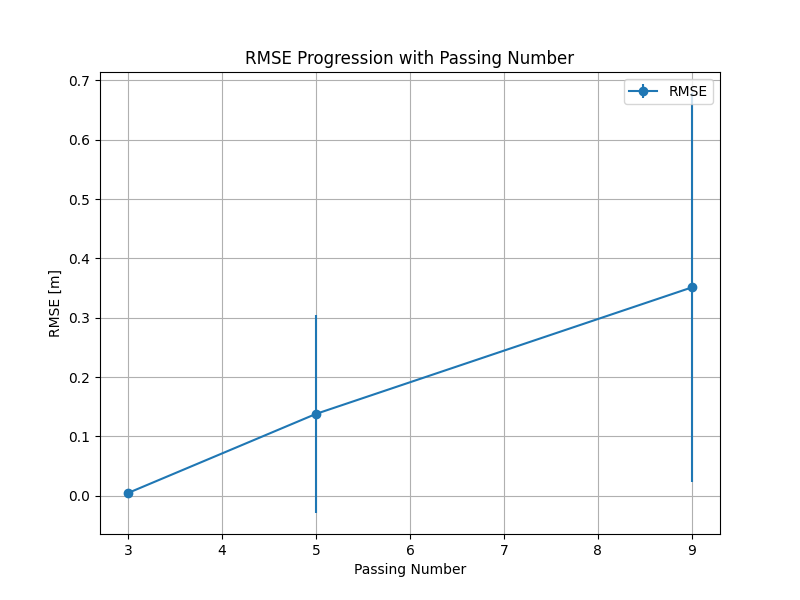
\includegraphics[width=0.95\textwidth]{Images/metrics_plots/10k/rmse_line_plot.png}
            \caption{RMSE against the number of message-passing layers}
            \end{figure}
            \column{0.5\textwidth}
        \begin{figure}
            \centering
            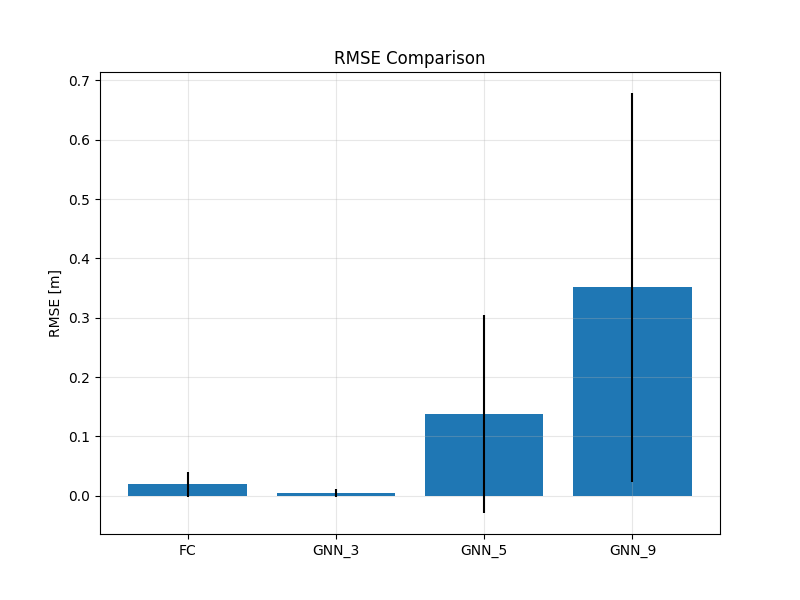
\includegraphics[width=0.95\textwidth]{Images/metrics_plots/10k/rmse_histogram.png}
            \caption{Comparison of the RMSE for the different models}
        \end{figure}
    \end{columns}
\end{frame}

\begin{frame}
    \frametitle{Numerical Results - Visualization}
    \begin{columns}
        \column{0.5\textwidth}
        \begin{figure}
            \centering
            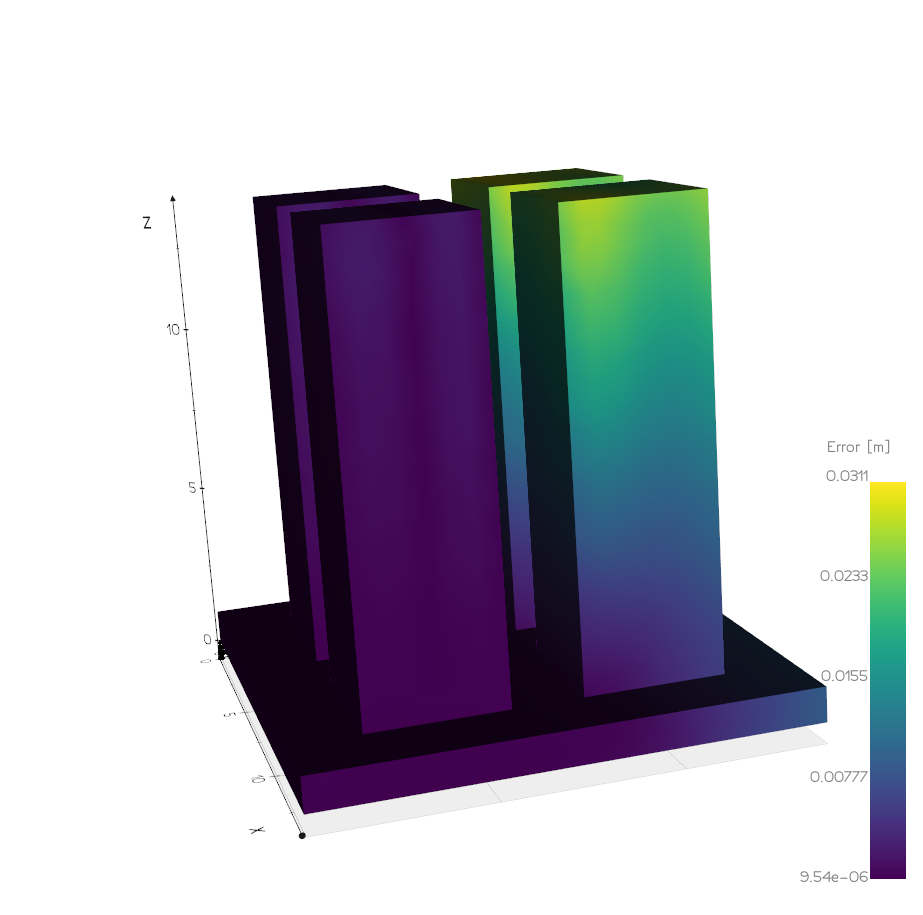
\includegraphics[width=0.95\textwidth]{Images/error_vis_3_pass_10k_1.png}
            \caption{Front view of the error}
            \end{figure}
            \column{0.5\textwidth}
        \begin{figure}
            \centering
            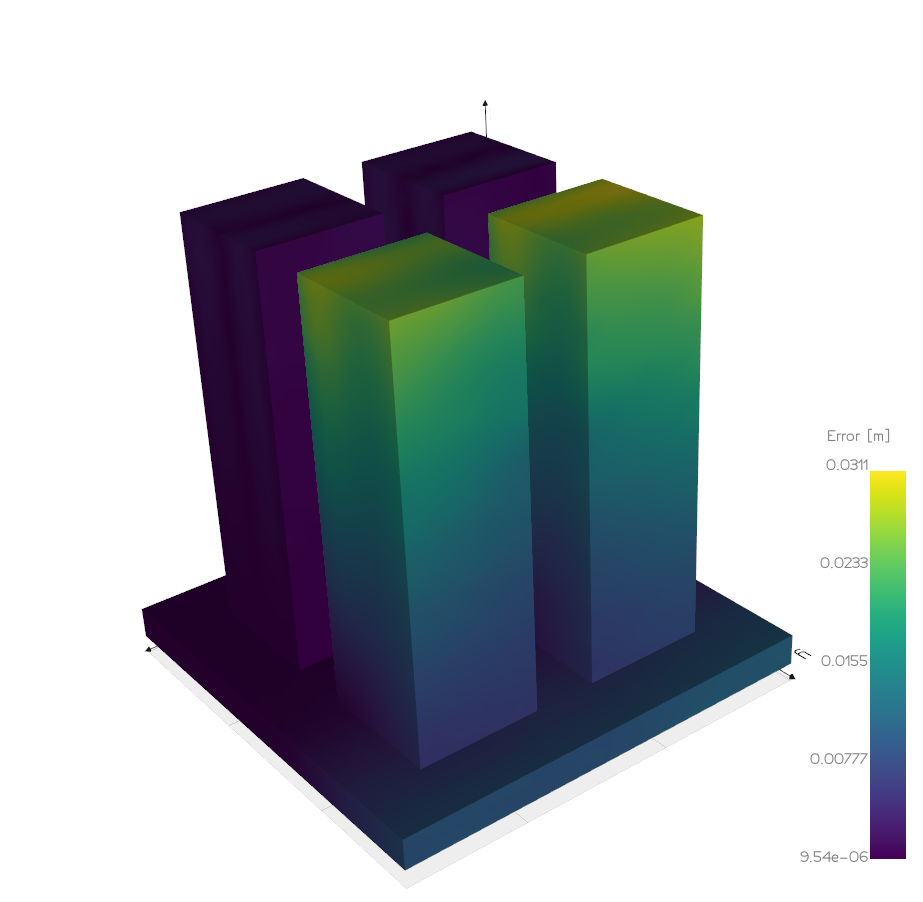
\includegraphics[width=0.95\textwidth]{Images/error_vis_3_pass_10k_2.png}
            \caption{Side view of the error}
        \end{figure}
    \end{columns}
\end{frame}

\begin{frame}
    \frametitle{Numerical Results - 5k dataset}
    Here are the results for the medium dataset (5000 simulations)

    \(9\) passing model not available because it's still training.
    \begin{table}
        \centering
        \begin{tabular}{|c|c|c|c|}
            \hline
            Model & RMSE (m) & MSE (m²) & RMSE (m) / L \\
            \hline
            GNN 3 MP & 0.0054 & 6.1e-05 & 0.0004 \\
            \hline
            GNN 5 MP & 0.1939 & 0.0946 & 0.0139 \\
            \hline
            GNN 9 MP & N/A & N/A & N/A \\
            \hline
            FC & 0.0216 & 0.0010 & 0.0015 \\
            \hline
        \end{tabular}
    \end{table}
\end{frame}

\begin{frame}
    \frametitle{Numerical Results - Visualization}
    \begin{columns}
        \column{0.5\textwidth}
        \begin{figure}
            \centering
            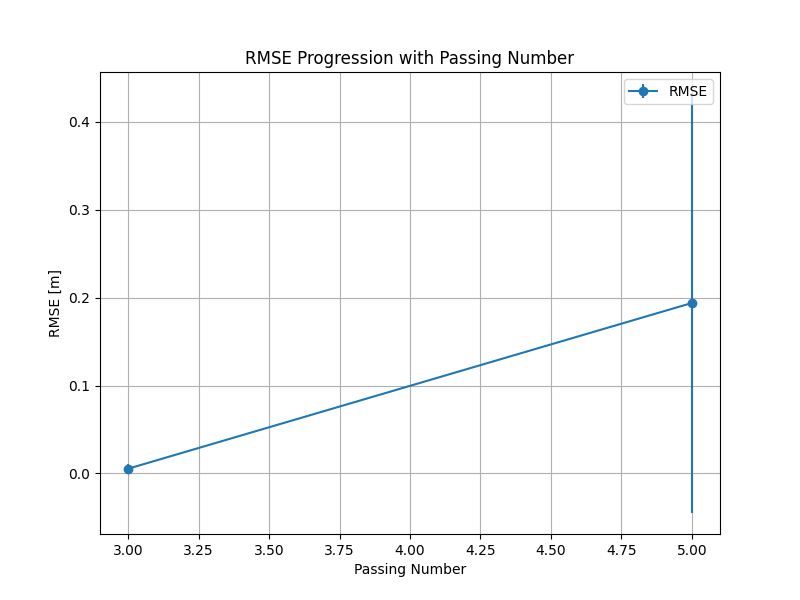
\includegraphics[width=0.95\textwidth]{Images/metrics_plots/5k/rmse_line_plot.png}
            \caption{RMSE against the number of message-passing layers}
            \end{figure}
            \column{0.5\textwidth}
        \begin{figure}
            \centering
            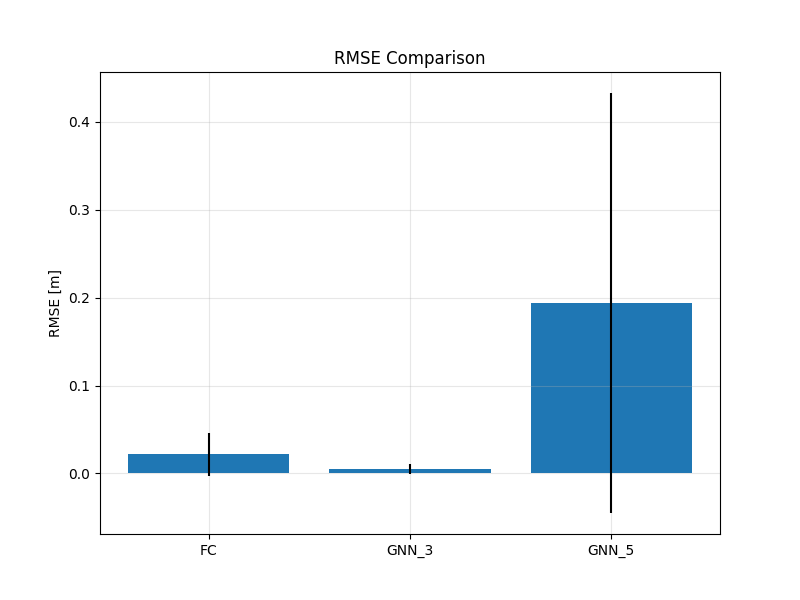
\includegraphics[width=0.95\textwidth]{Images/metrics_plots/5k/rmse_histogram.png}
            \caption{Comparison of the RMSE for the different models}
        \end{figure}
    \end{columns}
\end{frame}

\begin{frame}
    \frametitle{Numerical Results - 2k dataset}
    Here are the results for the small dataset (2000 simulations)

    \(9\) passing model not available because it's still training.
    \begin{table}
        \centering
        \begin{tabular}{|c|c|c|c|}
            \hline
            Model & RMSE (m) & MSE (m²) & RMSE (m) / L \\
            \hline
            GNN 3 MP & 0.0056 & 5.9e-05 & 0.0004 \\
            \hline
            GNN 5 MP & 1.3032 & 3.5762 & 0.093 \\
            \hline
            GNN 9 MP & N/A & N/A & N/A \\
            \hline
            FC & 0.0221 & 0.0011 & 0.0015 \\
            \hline
        \end{tabular}
    \end{table}
\end{frame}

\begin{frame}
    \frametitle{Numerical Results - Visualization}
    \begin{columns}
        \column{0.5\textwidth}
        \begin{figure}
            \centering
            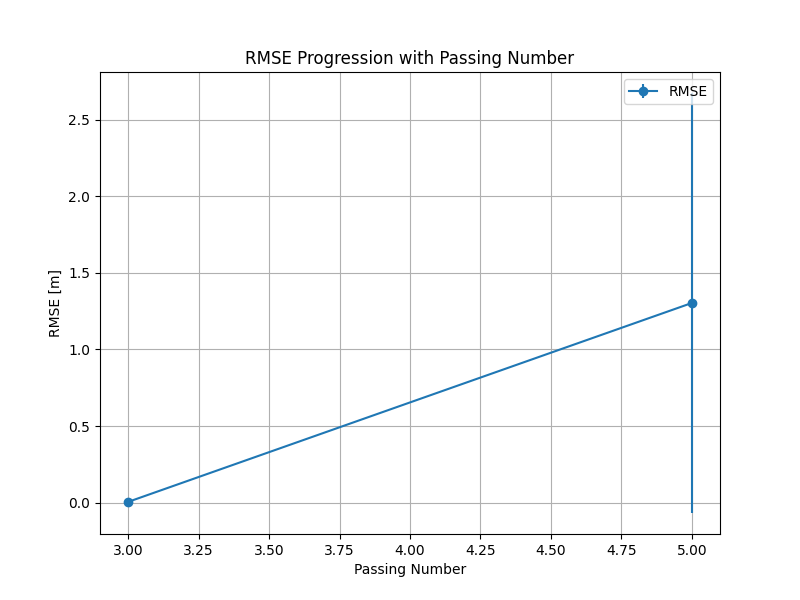
\includegraphics[width=0.95\textwidth]{Images/metrics_plots/2k/rmse_line_plot.png}
            \caption{RMSE against the number of message-passing layers}
            \end{figure}
            \column{0.5\textwidth}
        \begin{figure}
            \centering
            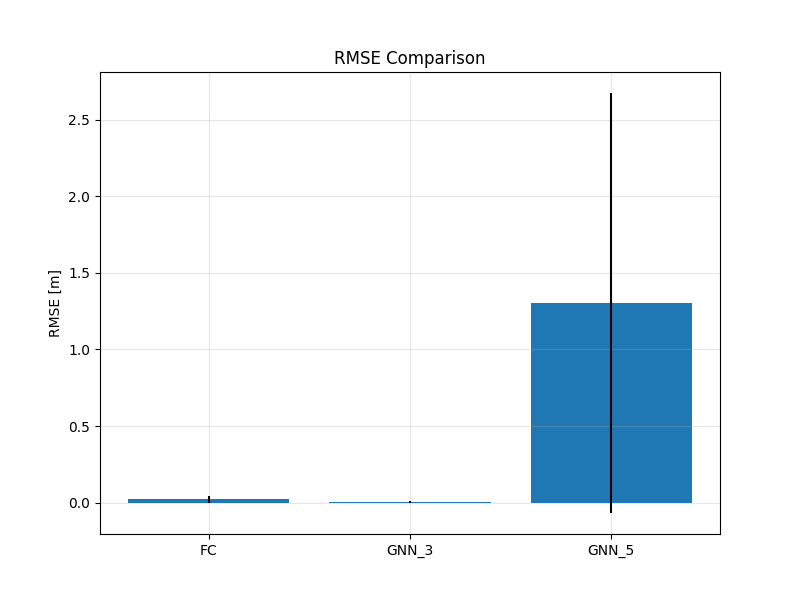
\includegraphics[width=0.95\textwidth]{Images/metrics_plots/2k/rmse_histogram.png}
            \caption{Comparison of the RMSE for the different models}
        \end{figure}
    \end{columns}
\end{frame}



\begin{frame}
    \frametitle{Conclusions}
    \begin{itemize}
        \item From the results, it seems like that increasing the number of message-passing layers decreases the accuracy of the model a lot.
        \item The size of the dataset seems to have a slightly positive effect on predictions, but maybe it is not worth the computational cost.
        \item This is clearly a worst case scenario in which the geometry is complex.
    \end{itemize}
\end{frame}


\begin{frame}
    \frametitle{Ideas}
    \begin{itemize}
        \item Explore different graph neural network architectures.
        \item Implement a loss function that takes into account the ``soundness'' of the solution.
        \item See what's the minimum amount of data needed to keep the model accurate.
        
    \end{itemize}
\end{frame}

%big centered text that says Questions and comments? in blue
\begin{frame}
    \begin{center}
        \Huge{\textcolor{blue}{Questions and comments?}}
    \end{center}
\end{frame}
\end{document}

